\documentclass{article}
 
\title{DIY Solar: Phone Chargers}
\author{Demand for Energy Equality}
\date{June 2019 \\ Root source version: Version 2.0 \\ Translation version: Version 0.1}

%inherited code
\usepackage{amsmath,amsthm,amssymb,epsfig}
\usepackage{hyperref}

% imports for images
\usepackage{caption}
% \usepackage[demo]{graphicx}
\usepackage{graphicx}
% \usepackage{float}

% import for resuming enumerated list
\usepackage{enumitem}

% code to remove numbering but keep the contents page filled
\setcounter{secnumdepth}{0}

\theoremstyle{definition}
\newtheorem{thm}{Theorem}[section]
\newtheorem{lem}[thm]{Lemma}
\newtheorem{prop}[thm]{Proposition}
\newtheorem{cor}[thm]{Corollary}
\newenvironment{pf}{{\noindent\sc Proof. }}{\qed}

\theoremstyle{definition}
\newtheorem*{defn}{Definition}
\newtheorem*{exmp}{Example}
\newtheorem*{prob}{Problem}
\newtheorem*{info}{Information}
\newtheorem*{warn}{Warning}
\newtheorem*{quest}{Question}
\newtheorem*{blockq}{Block Quote}
\newtheorem*{strong}{Strong}
\newtheorem*{code}{Code}
\newtheorem*{coderesult}{Code Result}

\theoremstyle{remark}
\newtheorem*{rem}{Remark}
\newtheorem*{note}{Note}
\newtheorem*{exer}{Exercise}

\setlength{\oddsidemargin}{0.25 in}
\setlength{\evensidemargin}{-0.25 in}
\setlength{\topmargin}{-0.6 in}
\setlength{\textwidth}{6.5 in}
\setlength{\textheight}{8.5 in}
\setlength{\headsep}{0.75 in}
\setlength{\parindent}{0 in}
\setlength{\parskip}{0.1 in}

%%%%%%%
% Some commonly used notation
%%%%%%%

\def\R{{\mathbb R}}
\def\X{{\mathcal X}}
\def\Y{{\mathcal Y}}
\def\E{{\mathbb E}}
\def\sign{{\rm sign}}

% END inherited code

\begin{document}
 
\maketitle{}

\begin{center}
  
\includegraphics[width=0.25\paperwidth]{../Images/image_0_0_(demand_energy_equality).png}
\end{center}

\begin{center}
  \includegraphics[width=0.45\paperwidth]{../Images/image_0_1_(solar_panel).png}
\end{center}

\vfill
  

\includegraphics[]{../Images/image_0_2_(license).png} \newline
This guide is provided under a \href{https://creativecommons.org/licenses/by-sa/4.0/legalcode}{Creative Commons BY-SA} license: \newline
Material may be freely shared and adapted under the following terms: You must give appropriate credit, provide a link to the license, and indicate if changes were made, and further distribution must be under the same license as the original.

\newpage

\tableofcontents

\newpage

\section{Preface} % (fold)
\label{sec:preface}

  \subsection*{Introduction} % (fold)
  \label{sub:introduction}
  
    This PDF has taken the content of the \href{https://www.demandenergyequality.org/build-your-own-panels}{"DIY Solar: Phone Chargers"} PDF and put them into a form which can be easily corrected, improved and translated by the community using LaTeX a markdown language for technical topics.

  % subsection introduction (end)

  \subsection*{Notes} % (fold)
  \label{sub:notes}

    Please note the modifications which have been made \& where you can find updates.

    \begin{enumerate}
      \item All the content of the PDF and put them into a form which can be easily corrected, improved and translated by the community using LaTeX a markdown language for technical topics.
      \item Any updates, corrections or translations to the PDF will be available at \href{https://github.com/darigovresearch/DIY-Solar-Phone-Chargers}{https://github.com/darigovresearch/DIY-Solar-Phone-Chargers} so do return periodically to check if you have the latest version.
      \item Modifications from the original work includes typo correction, card merging \& consistency consolidation (see the commit history for [en] for the specific changes if any).
    \end{enumerate}

    Feel free to share the PDFs and give the repository a star so more people are likely to see this work and can get the most out of it.

  % subsection notes (end)

  \subsubsection*{License} % (fold)
  \label{ssub:license}

    Unless otherwise specified, everything in this PDF is covered by the following licence:

    
\includegraphics[]{../Images/image_0_2_(license).png} \newline

    This work was based on the work \textbf{\textit{DIY Solar: Phone Chargers}} by \href{https://www.demandenergyequality.org/}{Demand Energy Equality}, licensed under a \href{https://creativecommons.org/licenses/by-sa/4.0/legalcode}{Creative Commons BY-SA}.

    To see this work in full go to \href{https://www.demandenergyequality.org/build-your-own-panels}{https://www.demandenergyequality.org/build-your-own-panels}
  
  % subsubsection license (end)

% section preface (end)

\newpage

\section{Introduction} % (fold)
\label{sec:introduction}

  \subsection{The Demand Energy Equality project} % (fold)
  \label{sub:the_demand_energy_equality_project}

    Demand Energy Equality (DEE) is a UK based community energy project that seeks to provide practical energy education using solar photovoltaics. We are a group working for systemic change in the way energy is produced, distributed, controlled, delivered and used. These aims are within the context of rising energy inequality (in the UK, at least), rising fuel bills, climate change and the increasing cost of fossil fuel extraction. See \href{https://www.demandenergyequality.org/about/}{our website} to find out more about the project.

    Through teaching people DIY solar PV skills we also aim to develop their relationship with energy, and enable them to understand it better: where it comes from, how it is used and how it relates to their demand and needs. Ultimately we aim for this to change behaviour, leading to better use of energy and overall reduced demand. Reduced energy use is an unavoidable fact of the relatively near future – far better to prepare now than be surprised later on.

  % subsection the_demand_energy_equality_project (end)
  
  \subsection{Using this guide} % (fold)
  \label{sub:using_this_guide}

    This written guide is for anyone interested in building their own solar phone charger, or learning more about the concepts involved. It assumes no prior knowledge of any kind relevant to building a fully functioning panel. The guide is designed to be used alongside other DIY guides and resources provided by DEE. 

    The guide starts with a summary of the tools and materials used. This is followed by a description of each of the steps in the process of building a portable 10W solar phone charger. At the end of the guide is an appendix with supplemental detailed information about the tools and materials needed. 

    For other types of DIY solar panel that can be made, \href{https://www.instructables.com/}{instructables.com} is a good place to start looking for alternative designs. DEE (and other organisations) run workshops based on other panel designs – you will find information about the \href{https://www.demandenergyequality.org/our-workshops/}{workshops} that we are currently running on the DEE website. 

    You will find the latest version of this guide available to download from the DEE website, as and when this guide is updated, alongside our \href{https://www.demandenergyequality.org/resources/}{other guides and resources}. 

    We encourage you to share the skills you learn with others through your own workshops, particularly if you are able to target and work with low-income communities. Please contact us for any support you feel you may need if you plan to do this.

  % subsection using_this_guide (end)

  \subsection{The design} % (fold)
  \label{ssub:the_design}

    The basic components of the design, and that which makes it economically and practically feasible are the “broken” solar cells. These are cells produced in the industrial manufacture process (mainly in China) that are broken either in transit, or during assembly on arrival. Because they are of no commercial use, these cells can be bought relatively cheaply.

    The solar charger this guide describes is a self-contained design, and can be connected directly to USB devices with no additional equipment needed. 

    This particular guide reflects the latest iteration in the construction of DIY photovoltaic panels as practiced by DEE, but it is likely that it may evolve and expand over time. Because we occasionally introduce new materials and construction methods, the guide may not always be in line with the other DIY resources published by DEE, and may not exactly reflect the content of current workshops. \href{https://www.demandenergyequality.org/contact-us}{Contact DEE} if you need an update on any recent changes. 
  
  % subsection the_design (end)
  
  \subsection{Disclaimer} % (fold)
  \label{sub:disclaimer}

    This guide is for general guidance only and whilst every effort is made to ensure that the information it contains is correct, it should not be relied upon as accurate. The information / advice contained within this guide is intended for use within the UK only and by persons of no less than 18 years of age. Use this guide at your own risk.
    
    DEE will not accept any liability for any loss, damage, injury or negligence direct or indirect from use of the information / advice contained within this guide.

  % subsection disclaimer (end)

  \newpage  

% section introduction (end)

\section{Before starting} % (fold)
\label{sec:before_starting}

  \subsection{Staying safe} % (fold)
  \label{sub:staying_safe}

    You should be aware of and familiarise yourself with any potential hazards involved in making a solar charger. Ensure you are working in a suitable environment - work indoors on a stable, clear surface, and make sure any trip hazards from trailing cables are cleared away. Have a source of water nearby for the emergency treatment of burns.

    Recognise that liquid flux is an irritant so avoid direct contact with your hands when using it and rinse off your hands asap once you’re done. If it gets in your eyes or mouth wash it out immediately.

    The main sources of danger are the soldering irons (DEE uses 80W irons that get significantly hotter than standard soldering irons). 

    \begin{itemize}
      \item handle soldering irons with care, making sure to never touch the hot metal parts. 
      \item do not grab an iron if it is dropped on the floor. 
      \item though the soldering irons have heat resistant cables it is possible to burn through them which would cause an electrical hazard.
      \item Always place the soldering iron back in the stand when not in use.
      \item put burns under running cold water for several minutes. 
    \end{itemize}

    The metal nozzles of heat guns can get very hot, especially on the high setting or with sustained use. They present similar safety issues as soldering irons. While using them, be careful not to point them towards people or anything that would be damaged by heat, and when finished with them always place the heat gun on its back or with the nozzle resting on a non-flammable surface (e.g. the tile on a soldering station).
  
  % subsection staying_safe (end)

  \subsection{Tools and materials} % (fold)
  \label{sub:tools_and_materials}

    To complete a solar charger you will ideally need

    \begin{itemize}
      \item a 40W-80W soldering iron with a flat tip, with a secure soldering stand with a damp sponge 
      \item a flat heatproof surface, e.g. a ceramic tile
      \item a flux pen – if these are refillable type they will need to be filled with liquid flux
      \item small wire cutters
      \item large household scissors
      \item small nose pliers
      \item a 2000W heat gun with high and low settings
      \item a flat head screwdriver
      \item a utility (Stanley) knife
      \item a multimeter set to measure DC voltage
      \item extra solder
      \item extra EVA
      \item a hot glue gun
      \item a grow lamp (optional, for indoor testing)
      \item heat-proof gloves (optional)
      \item a sheet of 4mm thick UV resistant polycarbonate, 350mm x 235mm, with 4mm holes drilled in each corner
      \item 0.5 Watt PV cells, approx 80mm x 40mm (25 cells should be enough, allowing for breakages)
      \item approx 2.5m of tabbing wire
      \item two sheets of EVA cut slightly larger than the polycarbonate sheet
      \item a sheet of thin plywood or other hard backing, 350mm x 300mm, with holes drilled to line up with the polycarbonate corner holes
      \item two small terminal blocks
      \item two 130mm lengths of 0.75sqmm wire
      \item A USB junction box (or small DC 12v-5v USB voltage converter)
    \end{itemize}

    See the Appendix for more info on how to source materials for a DIY solar panel.
  
  % subsection tools_and_materials (end)

  \subsection{How to Solder} % (fold)
  \label{sub:how_to_solder}

    This is the key skill that is needed to join solar cells together.

    Solar cells are connected together in series by soldering a length of tabbing wire from the front of one cell to the back of the next. Solar cells have white conductive strips on each side that tabbing wire can be soldered onto. 

    General tips for good soldering technique for solar cells:

    \begin{itemize}
      \item Make sure the tabbing wire is flat and straight – draw the wire between your fingers to flatten it.
      \item Remove dirt and oxidation by applying flux
      \item Ensure that the surfaces to be joined are heated to a sufficient temperature to allow the solder to flow (which is aided by the flux). This can be achieved by holding the soldering iron on a point to allow heat to build up until you can see the solder melting before moving the tip
      \item If using a chisel tip, hold the soldering iron vertically so that the flat tip has maximum contact with the tabbing wire (see photo below).
      \item Slowly draw the soldering iron along the tabbing wire (learning the right speed is a trial and error process). It should be possible to see the solder go shiny as it melts and then forms a wave as the soldering iron is drawn along the tabbing wire.
      \item Keep the soldering iron tip clean by wiping it on the wet sponge
    \end{itemize}

    \begin{figure}[!ht]
      \begin{minipage}{0.5\textwidth}
          \centering
          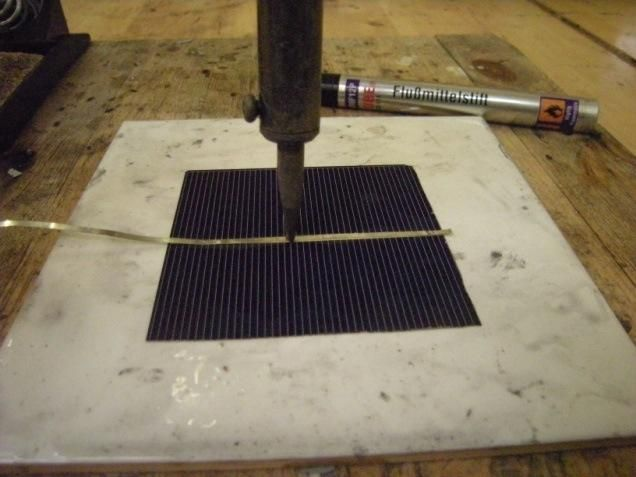
\includegraphics[width=0.9\textwidth]{../Images/image_2_1_(good_technique).png}
          \caption*{Good technique}
      \end{minipage}\hfill
      \begin{minipage}{0.5\textwidth}
          \centering
          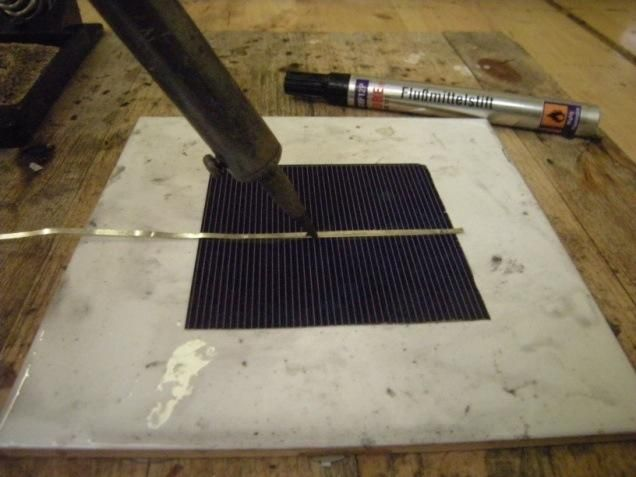
\includegraphics[width=0.9\textwidth]{../Images/image_2_2_(not_so_good_technique).png}
          \caption*{Not so good technique}
      \end{minipage}
    \end{figure}

    Common soldering errors:

    \begin{itemize}
      \item Forgetting to apply flux
      \item Moving the soldering iron too fast, not allowing enough time for the tabbing wire and cell below to heat up
      \item Not holding the soldering iron vertically
      \item Wiping the soldering iron repeatedly along the tabbing wire (this can remove the solder) – it is better to just do one slow stroke.
      \item Not cleaning the tip of the soldering iron regularly enough.
      \item Breaking cells by mishandling them or applying too much force with the soldering iron.
      \item Tabbing wire extending over the edge of the cell
    \end{itemize}
  
  % subsection how_to_solder (end)

% section before_starting (end)

\newpage

\section{Building the panel} % (fold)
\label{sec:building_the_panel}

  Summary of the construction process

  \begin{figure}[!ht]
    \begin{minipage}{0.25\textwidth}
        \centering
        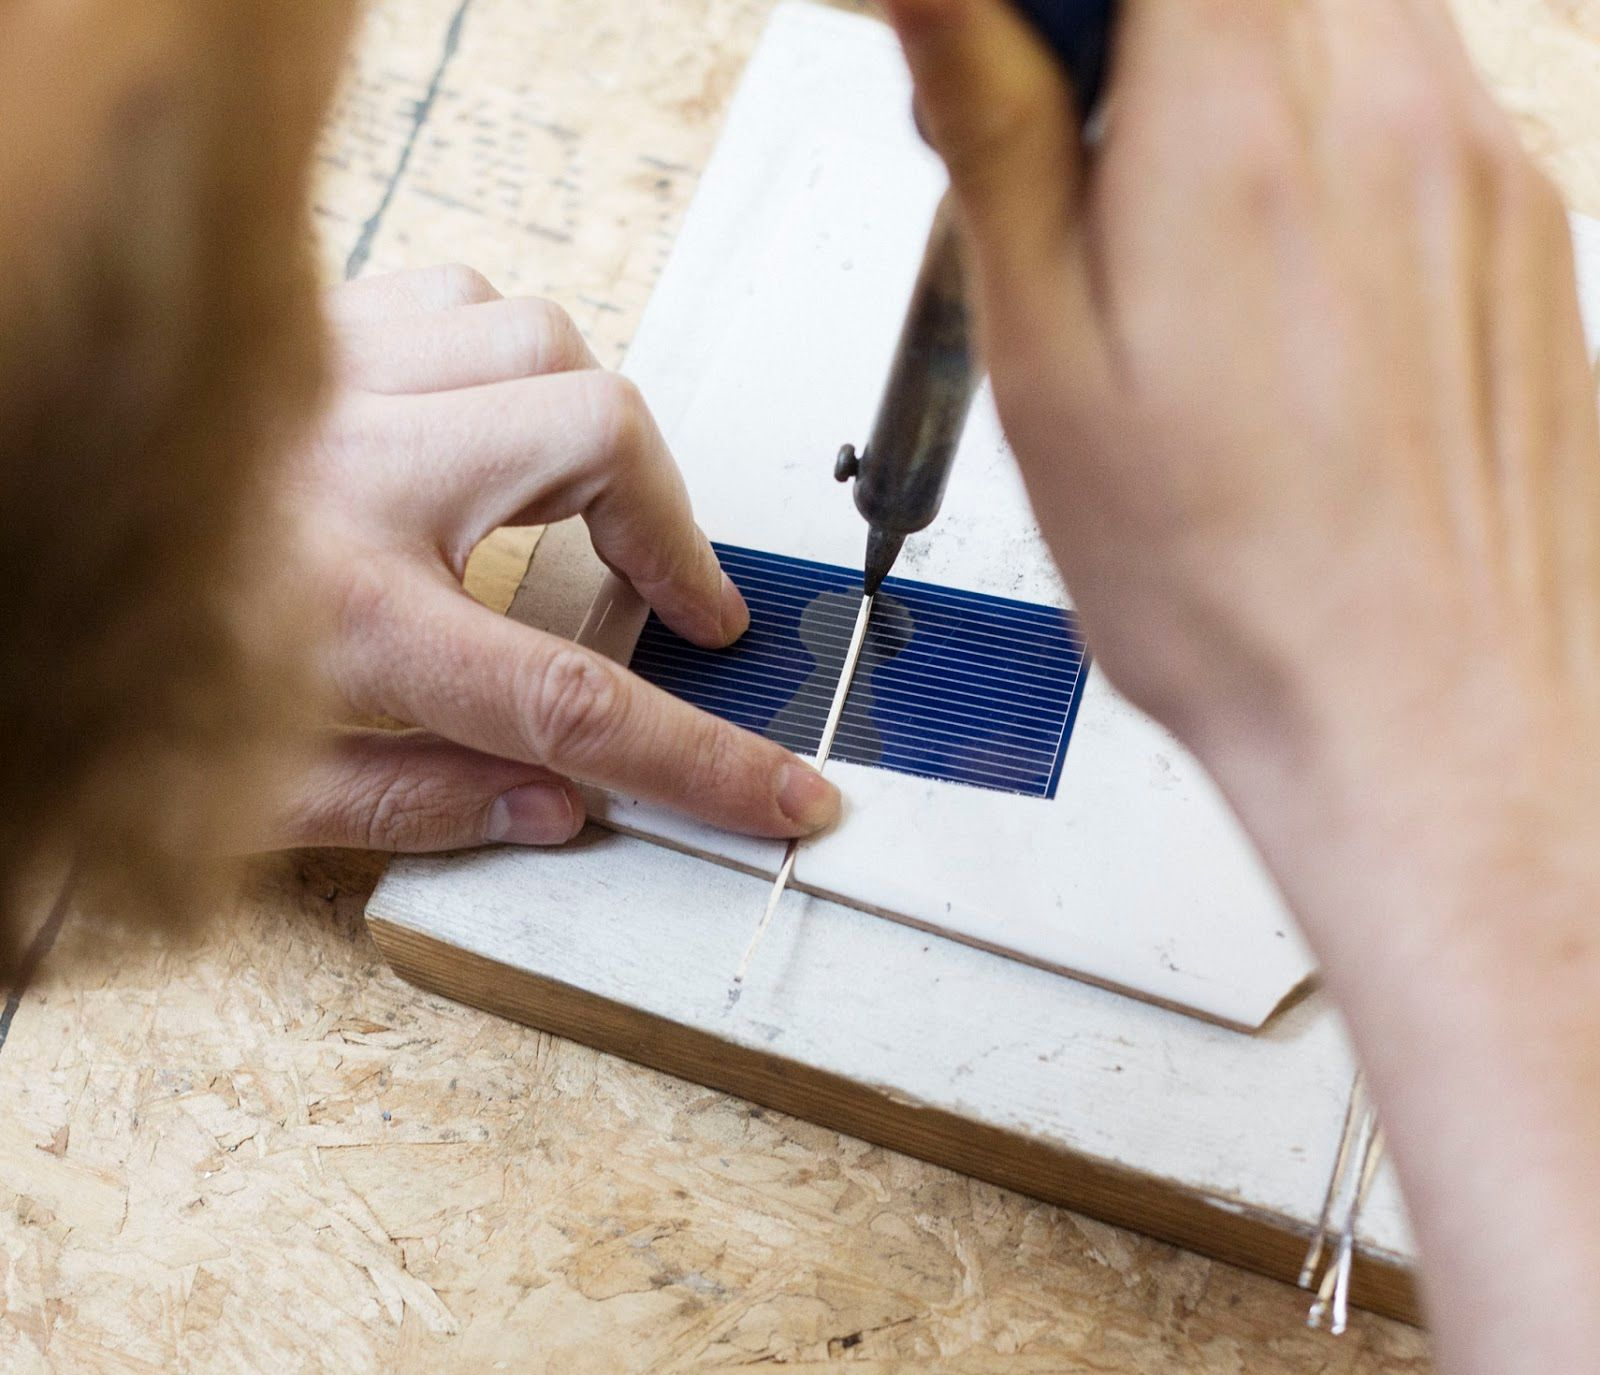
\includegraphics[width=0.8\textwidth]{../Images/image_3_1_(step_1).png}
        \caption*{Step 1: Solder tabbing wire to the top of cells}
    \end{minipage}\hfill
    \begin{minipage}{0.25\textwidth}
        \centering
        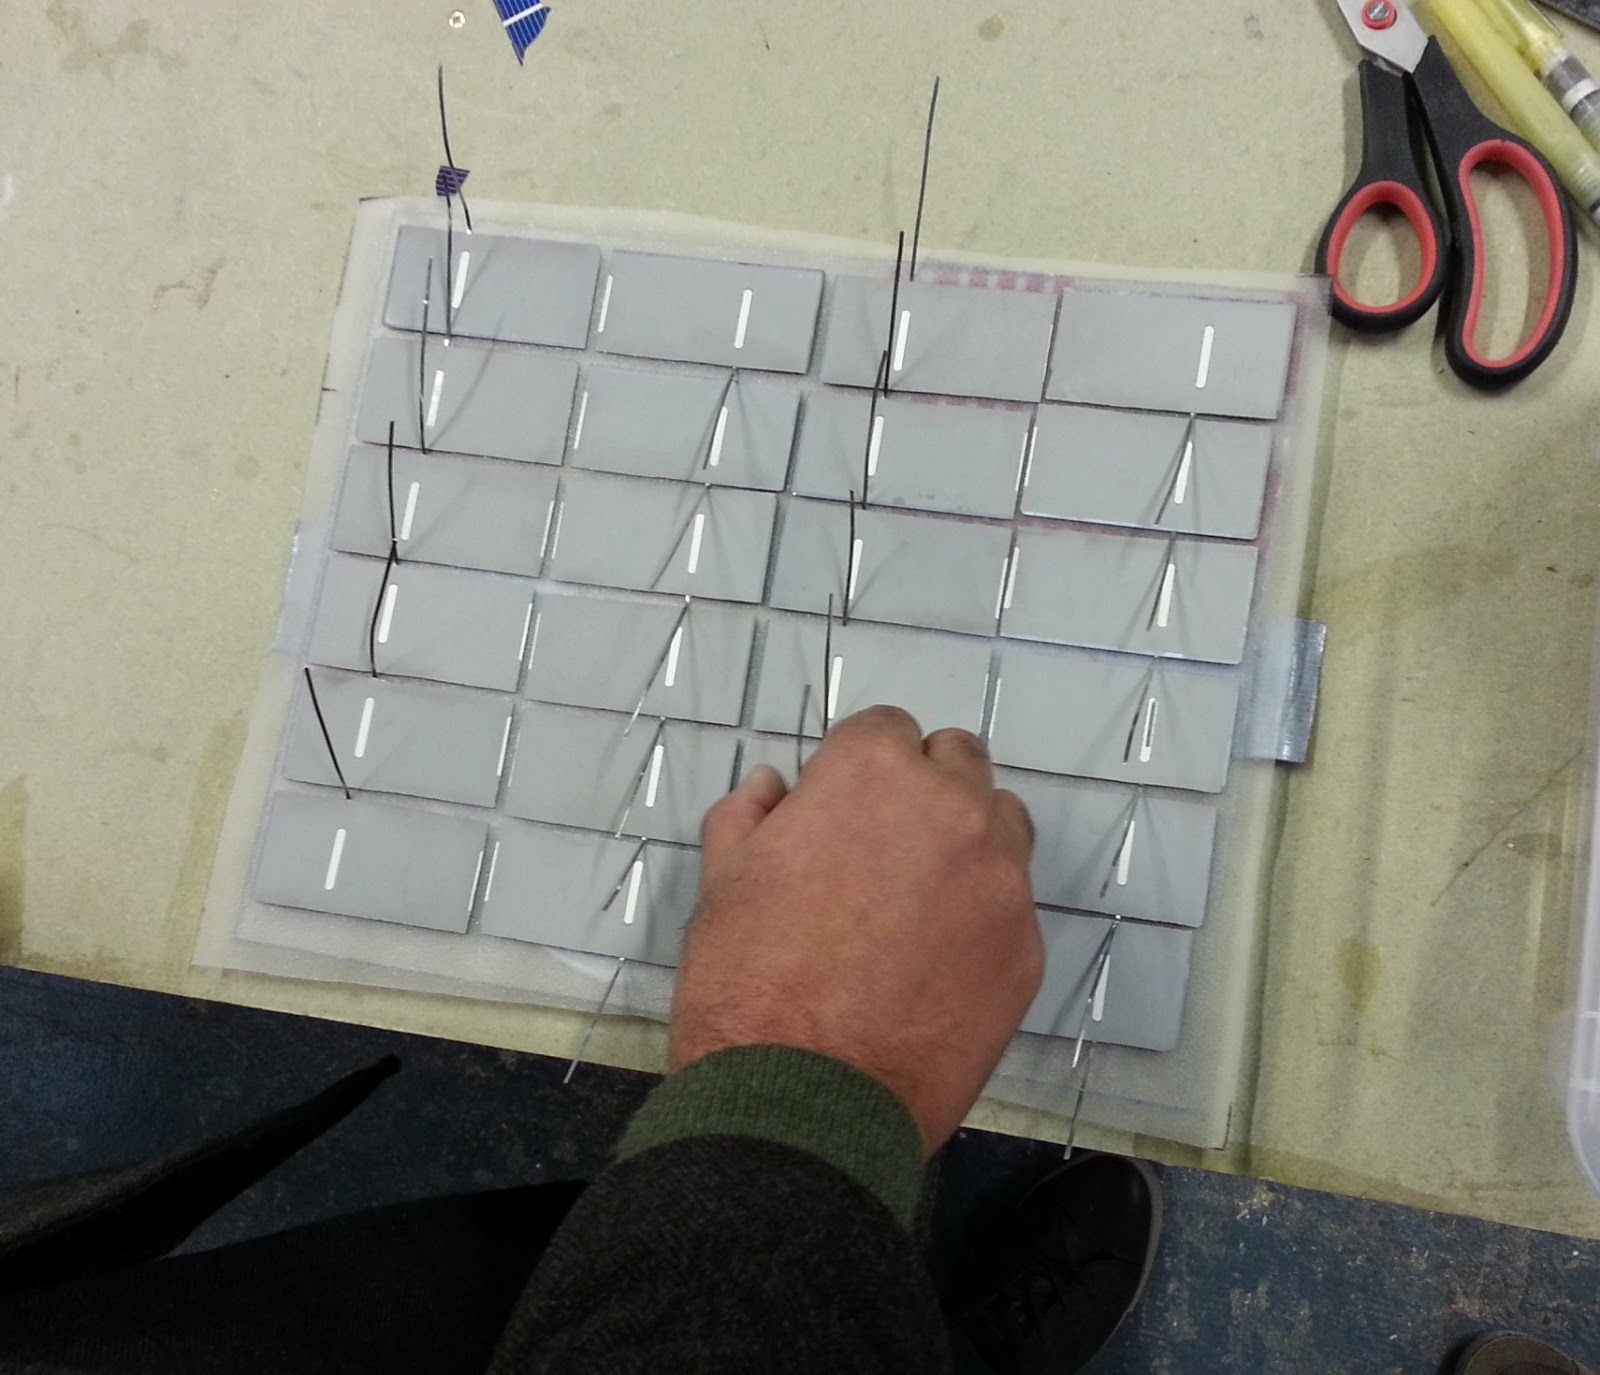
\includegraphics[width=0.8\textwidth]{../Images/image_3_2_(step_2).png}
        \caption*{Step 2: Lay EVA on polycarbonate sheet and arrange cells face down}
    \end{minipage}\hfill
    \begin{minipage}{0.25\textwidth}
        \centering
        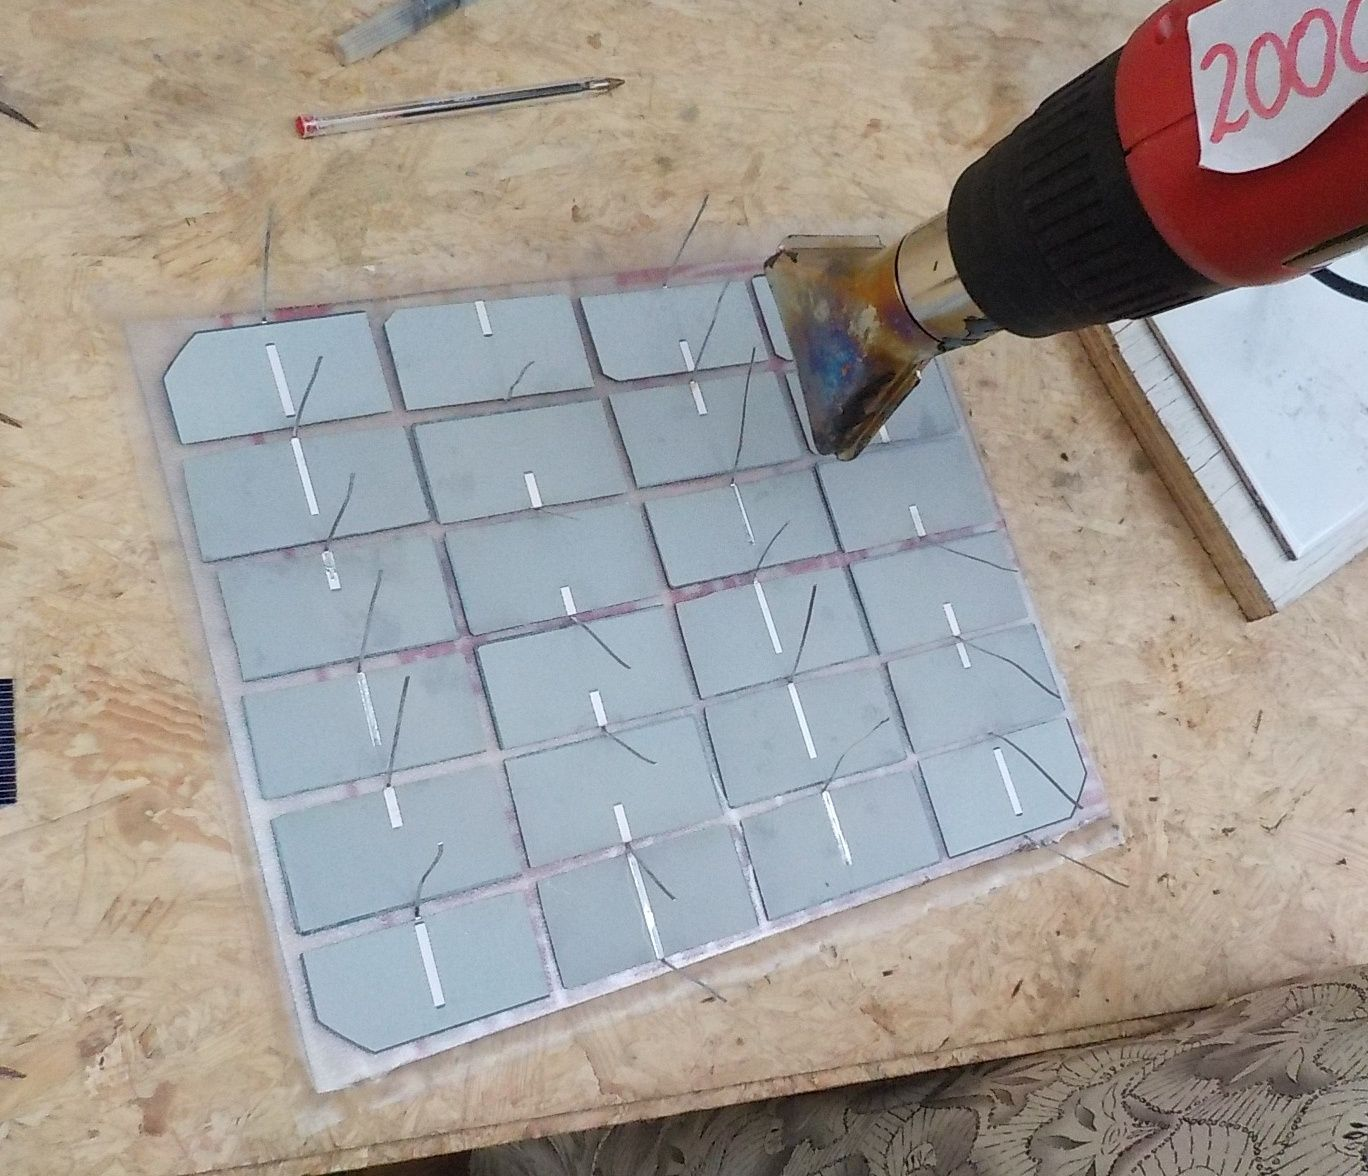
\includegraphics[width=0.8\textwidth]{../Images/image_3_3_(step_3).png}
        \caption*{Step 3: Apply enough heat to EVA to stick cells down}
    \end{minipage}
  \end{figure}

  \begin{figure}[!ht]
    \begin{minipage}{0.25\textwidth}
        \centering
        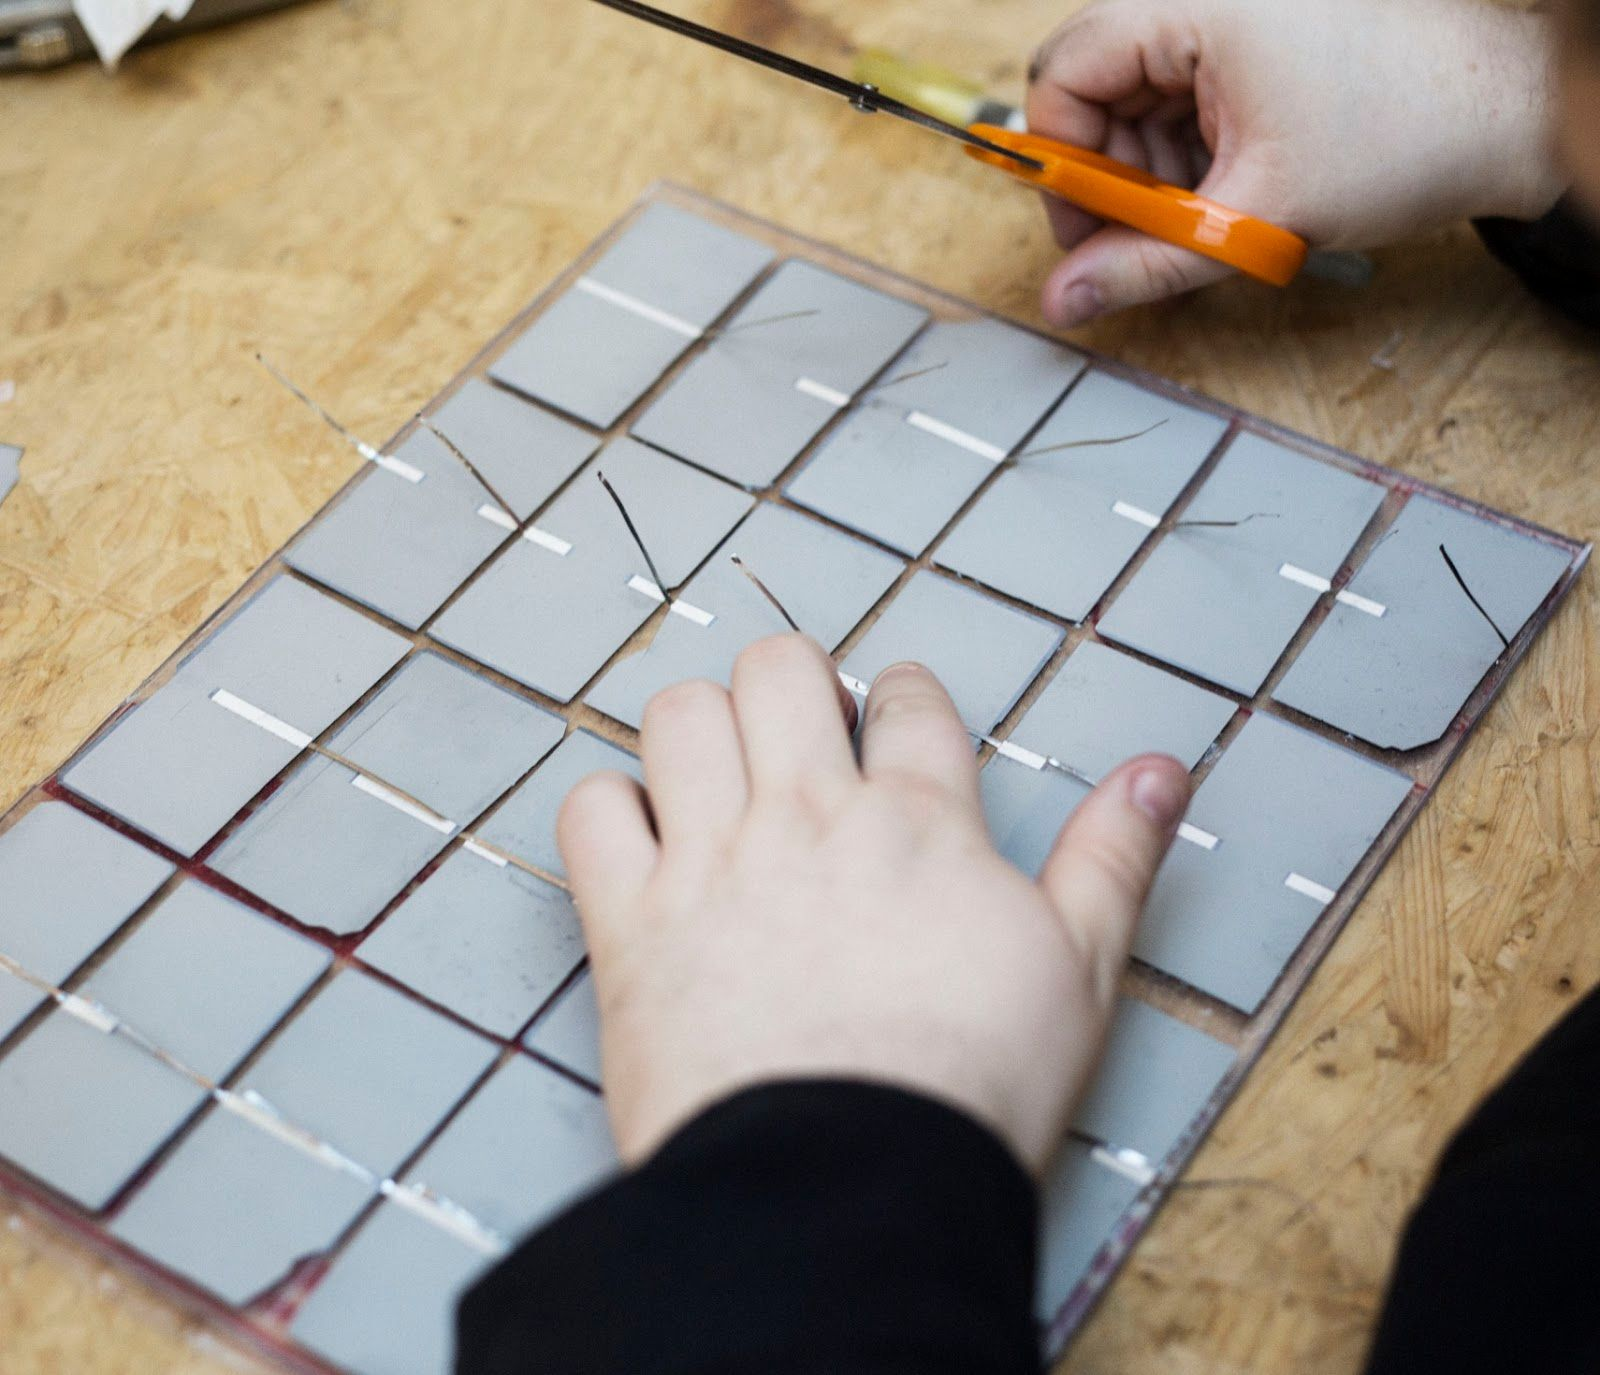
\includegraphics[width=0.8\textwidth]{../Images/image_3_4_(step_4a).png}
        \caption*{Step 4a: Tim tabbing wire tails  }
    \end{minipage}\hfill
    \begin{minipage}{0.25\textwidth}
        \centering
        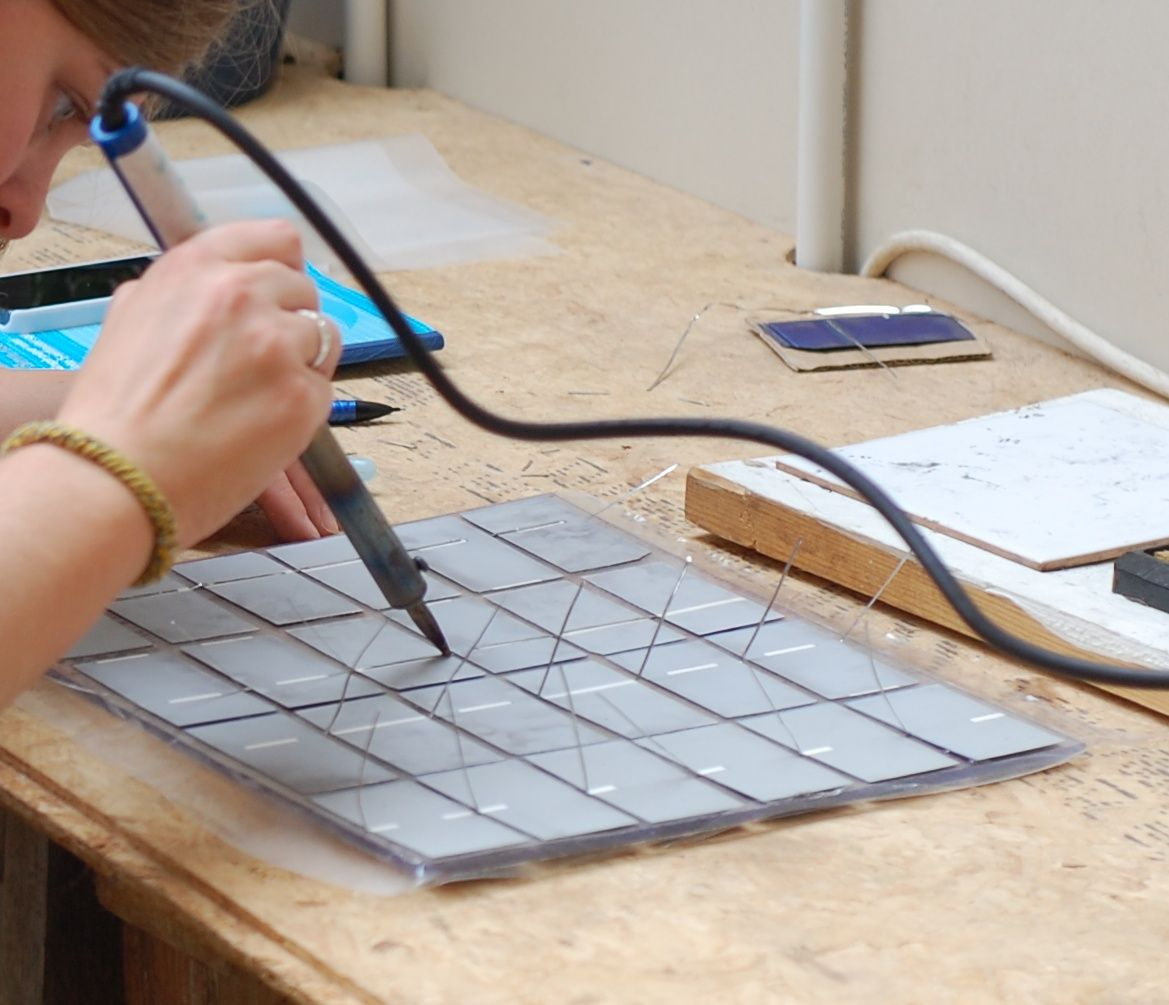
\includegraphics[width=0.8\textwidth]{../Images/image_3_5_(step_4b).png}
        \caption*{Step 4b: Solder tabbing wire tails to the backs of cells}
    \end{minipage}\hfill
    \begin{minipage}{0.25\textwidth}
        \centering
        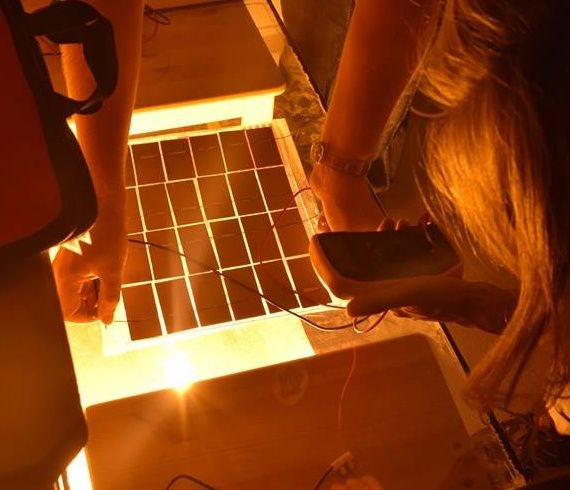
\includegraphics[width=0.8\textwidth]{../Images/image_3_6_(step_4c).png}
        \caption*{Step 4c: Test the voltage on each row and correct errors}
    \end{minipage}
  \end{figure}

  \begin{figure}[!ht]
    \begin{minipage}{0.25\textwidth}
        \centering
        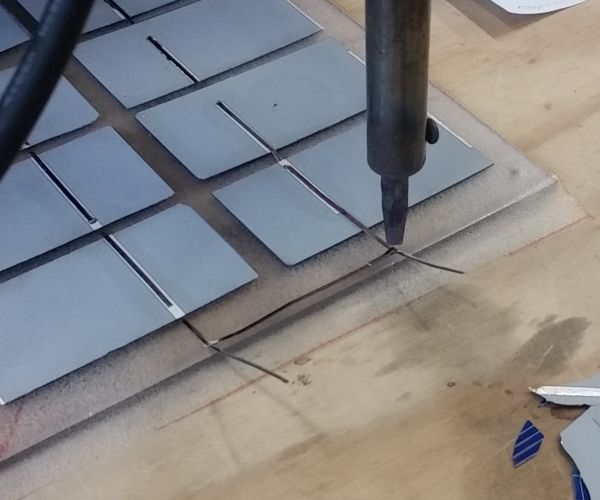
\includegraphics[width=0.8\textwidth]{../Images/image_3_7_(step_5a).png}
        \caption*{Step 5a: Connect rows together (cross-tabbing)}
    \end{minipage}\hfill
    \begin{minipage}{0.25\textwidth}
        \centering
        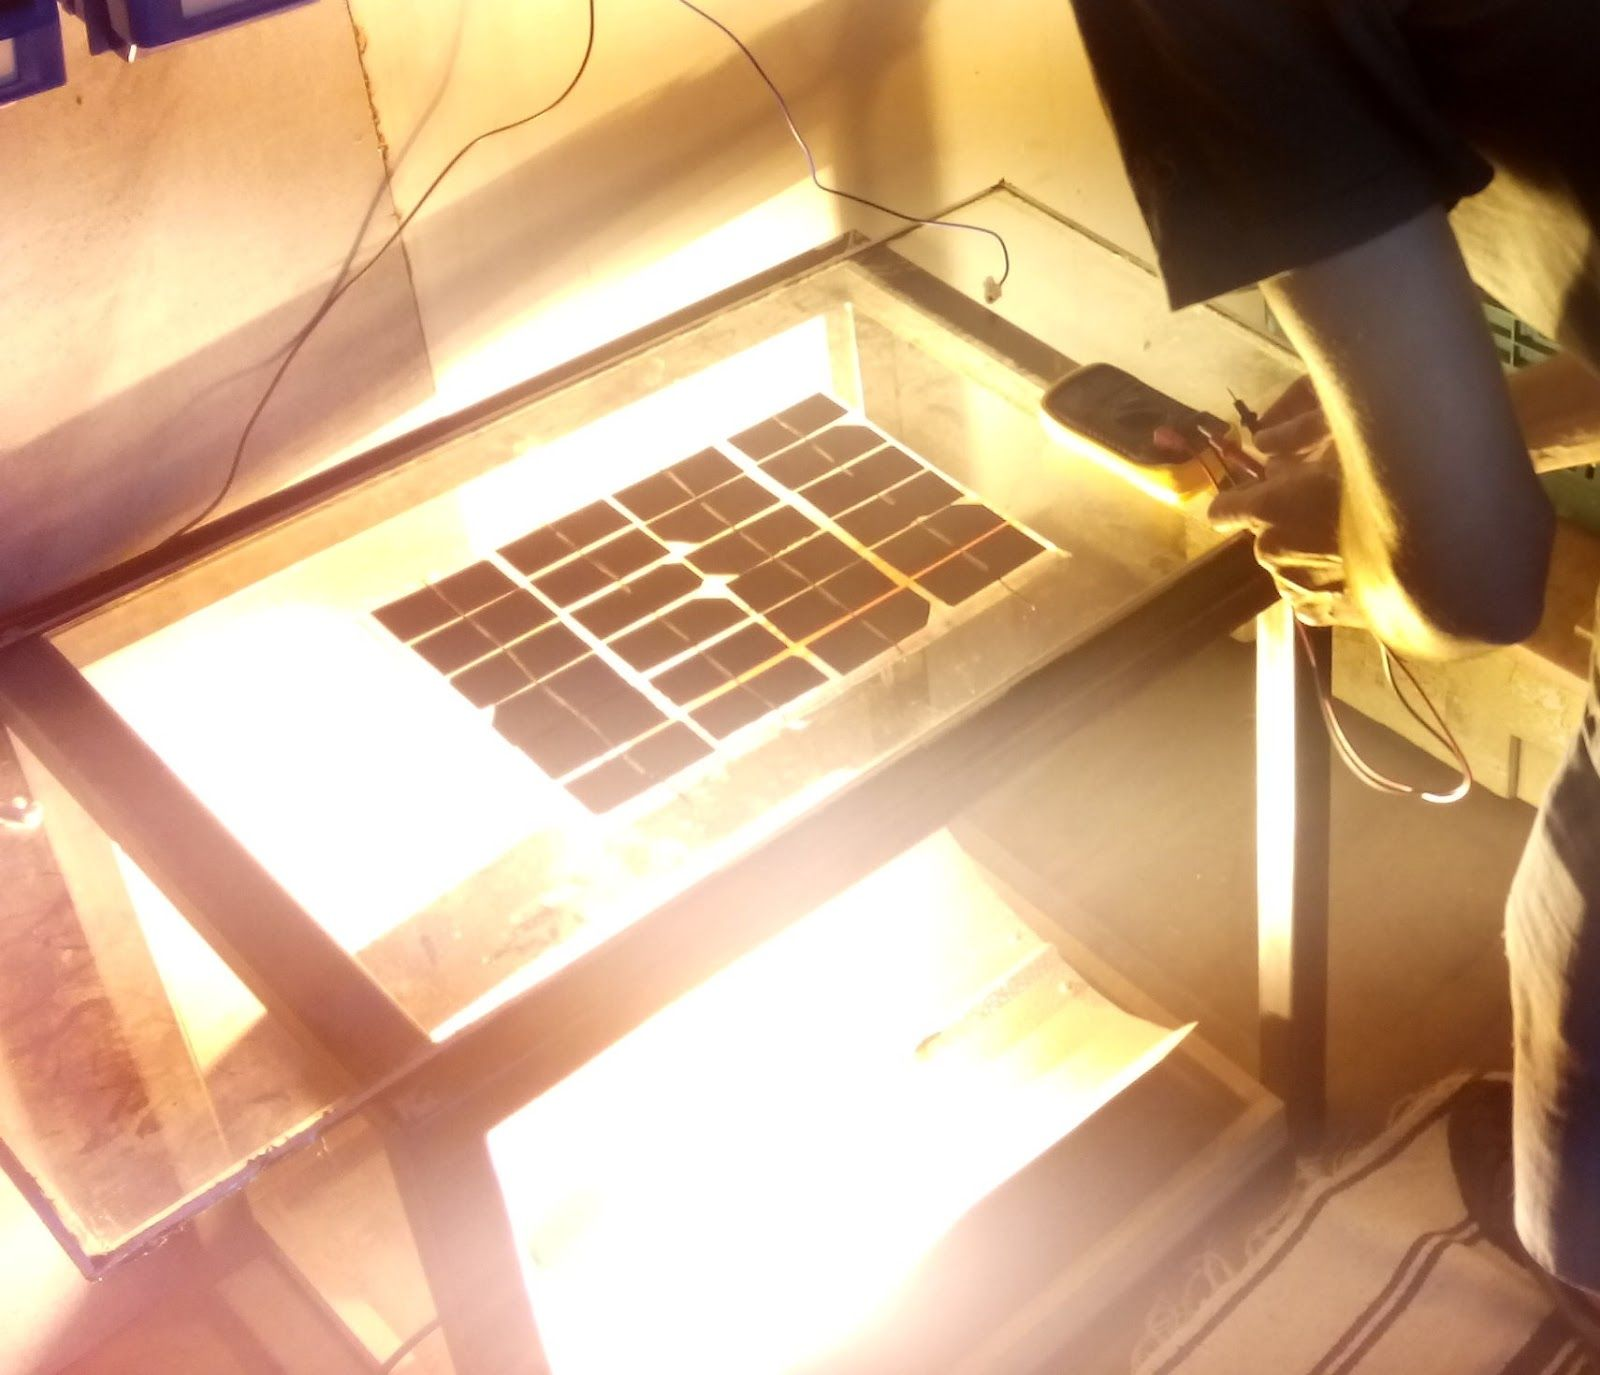
\includegraphics[width=0.8\textwidth]{../Images/image_3_8_(step_5b).png}
        \caption*{Step 5b: Test voltage and current of whole panel}
    \end{minipage}\hfill
    \begin{minipage}{0.25\textwidth}
        \centering
        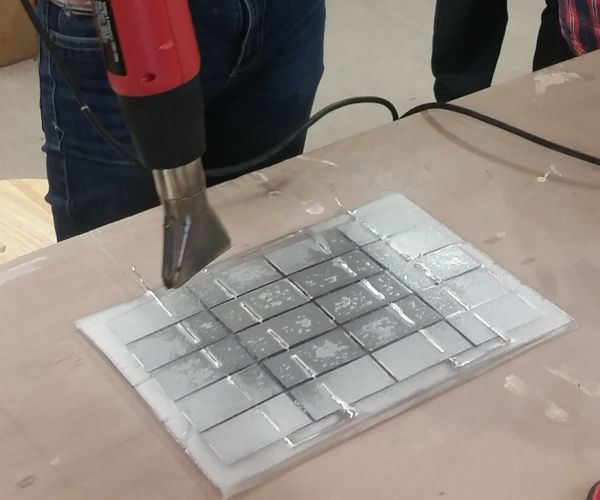
\includegraphics[width=0.8\textwidth]{../Images/image_3_9_(step_6).png}
        \caption*{Step 6: Encapsulate cells with second sheet of EVA}
    \end{minipage}
  \end{figure}

  \begin{figure}[!ht]
    \begin{minipage}{0.25\textwidth}
        \centering
        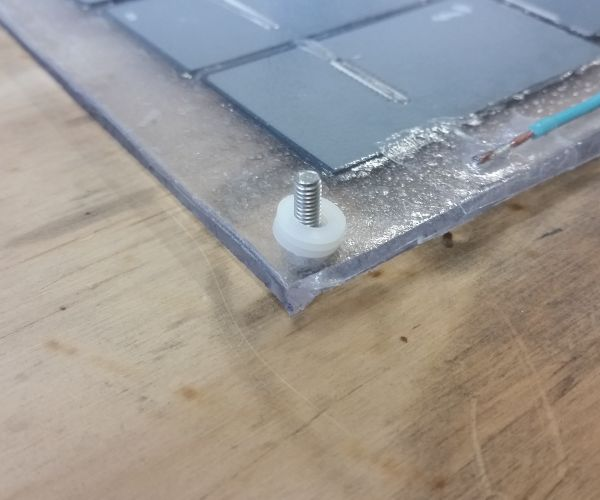
\includegraphics[width=0.8\textwidth]{../Images/image_3_10_(step_7).png}
        \caption*{Step 7: Mount solar panel onto hard backing with corner bolts}
    \end{minipage}\hfill
    \begin{minipage}{0.25\textwidth}
        \centering
        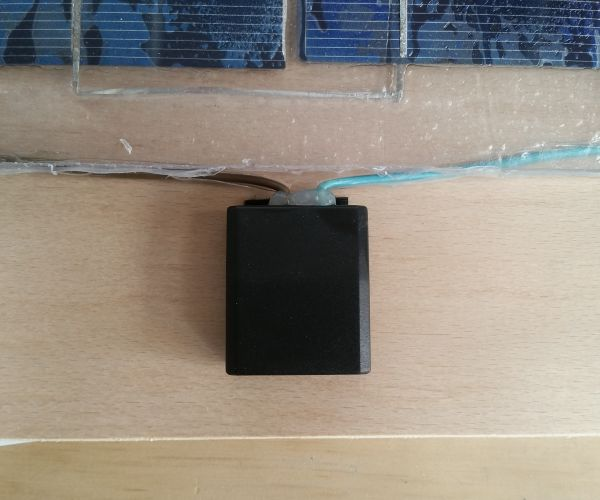
\includegraphics[width=0.8\textwidth]{../Images/image_3_11_(step_8).png}
        \caption*{Step 8: Attach USB junction box  Completed solar charger}
    \end{minipage}\hfill
    \begin{minipage}{0.25\textwidth}
        \centering
        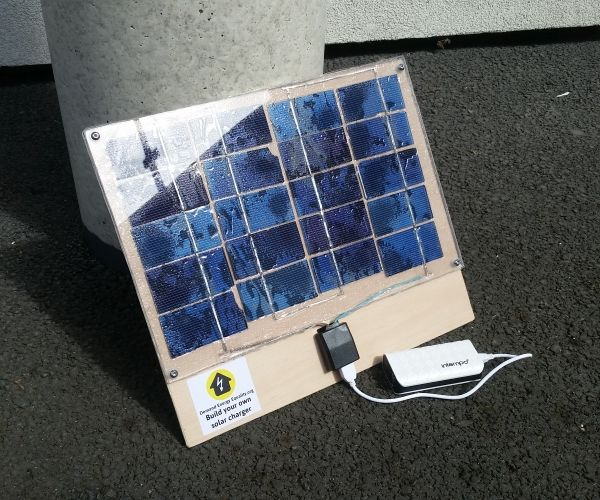
\includegraphics[width=0.8\textwidth]{../Images/image_3_12_(completed).png}
        \caption*{Completed solar charger}
    \end{minipage}
  \end{figure}

  \subsection{Step 1: Soldering tabbing wire to the top of the cells} % (fold)
  \label{sub:step_1_soldering_tabbing_wire_to_the_top_of_the_cells}

    You will need to become confident at soldering and build up a stock of cells with tabbing wire on one side. The first step is to solder an 80mm length of tabbing wire on to the thick white conductive strip on the front of the solar cell. Place the solar cell on the ceramic tile and lay the piece of tabbing wire over the white strip. The tabbing wire should be roughly twice the width of the solar cell, and you want to have a long ‘tail’ of wire running off the bottom of the cell. It’s important that the other end of the wire doesn’t hang over the edge of the top of the cell - always leave a couple of millimeters of clear space between the edge of the cell and the end of the wire. Each cell will generate 0.5V - you will need 20 of these to create a 10 volt panel.


    The tabbing wire tails from each cell will need to line up with the conductive contacts on the back of the next cell – some cells have their conductive strips off-set to one side, so make sure all the cells in a row all have their tails and conductive contacts in alignment.

    Additional spare cells can be soldered to replace possible breakages, to save time later.

    Tips

    \begin{itemize}
      \item Avoid soldering too close to the edge of the cell - loose solder on the edge of a cell can cause it to short circuit. 
      \item Putting too much pressure on the cells can cause them to crack. 
      \item If cell contacts are off-centre, make sure that the tabbing wire on all cells lines up when it comes to connecting them in columns.
    \end{itemize}
  
  % subsection step_1_soldering_tabbing_wire_to_the_top_of_the_cells (end)

  \subsection{Step 2: Preparing the polycarbonate and placing the cells} % (fold)
  \label{sub:step_2_preparing_the_polycarbonate_and_placing_the_cells}

    Place one sheet of EVA on the polycarbonate (remove any protective film first). Arrange the tabbed cells face down on the panel in 4 rows of 5 cells, with the tails bent so that they point slightly up. There should be a clearly visible gap between each cell (~ 2mm) and a gap at the top and bottom of each row (~ 5-10mm). It can be useful to have a grid drawn out on a sheet of paper to aid the correct arrangement of the cells. The direction of cells in each column should alternate, so that they can be connected in series to create a continuous string (or “snake”). 

    You may need to cut/trim sheets of EVA to use – they should be slightly larger than the polycarbonate sheets, with a margin of around 5mm on each edge. You will need two of these sheets, so it’s advisable to cut them both at the same time.

    Tips

    \begin{itemize}
      \item Avoid shorting the circuit by not having cells touching each other.
      \item Check that rows of cells are running in opposite directions – failure to do so can waste a lot of time and materials.
      \item Check that contact points for soldering tabbing wire tails are all lined up properly.
      \item Check each cell for cracks or poor soldering before placing it
    \end{itemize}
  
  % subsection step_2_preparing_the_polycarbonate_and_placing_the_cells (end)

  \subsection{Step 3: Heating the EVA to stick the cells} % (fold)
  \label{sub:step_3_heating_the_eva_to_stick_the_cells}

    This step involves sticking cells to the sheet of polycarbonate using heated EVA. Use the low setting on your heat gun to apply heat to the cells and the EVA. As it heats the EVA should turn transparent and become tacky. If the EVA is creased or folded, it may be necessary to carefully apply a little pressure to the edges of each cell as they heat up to make sure they are stuck flat on the polycarbonate. Once the heat is removed, the EVA will cool and cells will remain bonded. It's not necessary to apply a lot of heat at this stage – just enough to fix the cells in place to allow the tabbing wire tails to be soldered. Give the tail of each cell a slight wiggle to check it is fixed in place.

    Tips

    \begin{itemize}
      \item If cells crack after they've been stuck down, you will need to use the heat gun to loosen the EVA bond before you can remove the broken cell. If the cell is removed while the EVA is cool, it will fragment into lots of tiny pieces which are time-consuming to remove. 
      \item The easiest way to remove a broken cell is to use a thin blade to carefully lift the cell off once the EVA is hot.  
      \item Once a cell has been removed, you may need to use an extra patch of EVA to fill any holes – it's useful to have some spare EVA offcuts available for this purpose.
      \item Overheating can cause cells to be overly stuck down and then difficult to remove later
    \end{itemize}

    A note on cracks

    Everyone who builds solar panels breaks cells at some point and this is a guide to whether to replace cells that get cracked. Early in the construction process before cells are stuck down and connected together you can afford to be fairly conservative and to discard most cells that get cracked. But once they are connected together it is a time consuming job to strip off the tabbing wire and to remove the cell. This a quick visual guide to help you decide whether to replace a cracked cell.

    \begin{figure}[!ht]
      \begin{minipage}{0.45\textwidth}
          \centering
          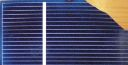
\includegraphics[]{../Images/image_3_13_(less_than_10_percent).png}
          \caption*{Less than 10\% broken off – \textbf{OK}}
      \end{minipage}\hfill
      \begin{minipage}{0.45\textwidth}
          \centering
          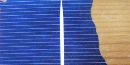
\includegraphics[]{../Images/image_3_14_(more_than_10_percent).png}
          \caption*{More than 10\% broken off - \textbf{REPLACE}}
      \end{minipage}
    \end{figure}

    \begin{figure}[!ht]
      \begin{minipage}{0.45\textwidth}
          \centering
          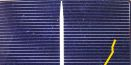
\includegraphics[]{../Images/image_3_15_(minor_crack_away_from_strip).png}
          \caption*{Minor crack away from conductor strip – \textbf{OK}}
      \end{minipage}\hfill
      \begin{minipage}{0.45\textwidth}
          \centering
          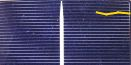
\includegraphics[]{../Images/image_3_16_(minor_horizontal_crack).png}
          \caption*{Minor horizontal crack - \textbf{OK}}
      \end{minipage}
    \end{figure}

    \begin{figure}[!ht]
      \begin{minipage}{0.45\textwidth}
          \centering
          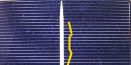
\includegraphics[]{../Images/image_3_17_(long_crack_parallel).png}
          \caption*{Long crack parallel to conductor strip – if the crack propagates half the cell would be lost - \textbf{REPLACE}}
      \end{minipage}\hfill
      \begin{minipage}{0.45\textwidth}
          \centering
          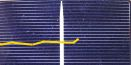
\includegraphics[]{../Images/image_3_18_(long_crack_across).png}
          \caption*{Long crack across conductor strip – this is \textbf{OK} providing there is tabbing wire across the crack on both sides (it effectively becomes a parallel connection) but check for shorting}
      \end{minipage}
    \end{figure}

  % subsection step_3_heating_the_eva_to_stick_the_cells (end)

  \subsection{Step 4: Tabbing the other side of the cells} % (fold)
  \label{sub:step_4_tabbing_the_other_side_of_the_cells}

    Once the tabbed cells are stuck to the polycarbonate the tails can be soldered onto the backs of adjacent cells to connect them in series. You should now trim any excess tabbing wire on each tail using small wire cutters - any wire that extends beyond the contact on the back of the adjacent cell isn’t needed, and wires should end a few mm short of the edge of the cell. Solder each tabbing wire tail to the back of the next cell, using a similar technique as on the front of the cell. Since the tabbing wire tails will try to spring up when being soldered, you can use the tip of a screwdriver or some other heat-proof implement to hold them in place while they are being soldered. Leave the tails coming off the end of each row, and cells at the other end of each row will need an extra strip of tabbing wire soldered to their backs.

    Tips

    \begin{itemize}
      \item Avoid shorting the circuit by not soldering too close to the edge of the cell, and avoid putting too much pressure on the cells as they are likely to crack. 
      \item If cells crack at this stage, they will need to be de-soldered from adjacent cells before they can be removed from the EVA as above.
      \item Check tabbing wire tails are firmly soldered to the back of cells by using a fingernail to try to lift them. Any weak connections that are not spotted at this stage are likely to fail when the cells are encapsulated.
      \item Using a multimeter and a light source to test each row of cells before moving on to the next stage can allow you to spot and fix problems early.
      \item GO SLOWLY as breakages now are very hard to fix
    \end{itemize}

    TODO ADD BOX

    Testing the pane

    Testing is best done in bright sunshine outside but in some circumstances it can be carried out over a high wattage grow lamp placed under a glass-topped table. 

    Use a multimeter set to measure DC voltage, on the 20V setting. With the solar panel pointing towards the light source, touch the probes on the multimeter to the tabbing wire coming off each end of a row to measure the voltage it is generating. Each row of 5 cells should measure around 2.5 volts. If you are measuring less than that, it may be because there is not enough light for testing, or that one or more cells is short circuited. Touch the probes to the tabbing wire running either side of a cell to measure the voltage of each individual cell - if any of those is reading 0 volts, it is short circuited. If the entire row is reading 0 volts, there is a bad connection - go over each soldered contact on each cell to make sure the connections are good, and test again.

    You can also use the multimeter to check the polarity of each row - touching the positive probe to the positive side of the row and the negative probe to the negative side of the row will give a positive result - reversing the probes will give a negative result.
  
  % subsection step_4_tabbing_the_other_side_of_the_cells (end)

  \subsection{Step 5: Cross tabbing} % (fold)
  \label{sub:step_5_cross_tabbing}

    Before starting, identify the positive and negative terminals of your solar panel, which will be on the same edge of the panel coming from the end cell of the outer rows. This will determine the rows that need to be connected to create a continuous ‘snake’ of cells. A piece of tabbing wire is used to connect across each row. To keep the cross tabbing secure, but also allow access to it in the event of a problem, the cross-tabbing should run between rows just inside the edge of the polycarbonate. 

    Take a piece of tabbing wire that is around 10mm longer than the distance between the tails on the rows that need to be connected and lay it under them. With the cross-tabbing wire in position, fold the ends very tightly up and around each tail, crimping the joint with a pair of small-nosed pliers if necessary. Hold the free end of one of the tails, lifting it up very slightly to keep it off the plastic underneath. Use a soldering iron to melt the solder on both wires together - this should only take around 5 seconds. Give the cross-tabbing wire a gentle tug to check that it is firmly connected. Repeat for the other tail. 

    Once the rows have been connected, you should have a continuous series of cells, with two free lengths of tabbing wire remaining at each end. These are the terminal wires, and should be left extending out from the polycarbonate sheet. One is the positive terminal, and the other is the negative.

    Optional - you can also solder short (~5cm) lengths of flex wire to the positive and negative terminals of the panel.

    Tips

    \begin{itemize}
      \item Make sure not to connect the tops and bottoms of two rows together to create a loop. 
      \item Optional - use the end of a pair of scissors under the cross tabbing joints when soldering to provide a firm base and avoid melting the polycarbonate. 
      \item Make sure to test the output of the whole panel before moving on to the next stage (see Testing the panel above). You should get a reading of at least 10 volts.
    \end{itemize}

  % subsection step_5_cross_tabbing (end)

  \subsection{Step 6: Encapsulation} % (fold)
  \label{sub:step_6_encapsulation}

    Use a second sheet of pre-cut EVA, placed over the backs of the cells to encapsulate the panel. Encapsulation seals the cells from air and water intrusion, and prevents failure due to galvanic corrosion. Use the heat gun on a high setting to seal the cells and tabbing wires, applying heat evenly to the whole panel. It usually takes around 5 mins to get the EVA up to the right temperature, by which point it will look clear and glossy, and will be very sticky to touch.

    Once this has been done, leave the panel to cool for a couple of minutes, then use a pair of scissors to trim any excess EVA around the edge of the panel - making sure not to cut the tabbing wires.

    Tips

    \begin{itemize}
      \item All cells should be totally encapsulated – make sure there are no edges sticking out.
      \item The application of heat at this stage may break poorly soldered connections as the metal expands – this can cause the panel to perform poorly, or even break it entirely. It's very important to ensure all soldered connections are good before this stage. 
      \item When using the high heat setting, ensure that the heat gun is constantly moving to avoid creating a hot spot and warping the polycarbonate.
      \item The colder the environment you’re working in, the longer it will take to heat up the EVA, so if you’re working in a cold space, add more time for this step.
    \end{itemize}
  
  % subsection step_6_encapsulation (end)

  \subsection{Step 7: Bonding the panel into the neoprene case} % (fold)
  \label{sub:step_7_bonding_the_panel_into_the_neoprene_case}

    At this point, the panel can be mounted onto a hard backing using small corner bolts. Our design uses 5.5mm plywood sheets, and 4mm bolts. 

    Use wire cutters or a sharp knife or the tip of a small screwdriver to create a hole in the EVA over the corner holes. Keeping the panel face down to protect the cells, insert a bolt from beneath through each hole. Place 2 nylon washers over each bolt - these act as spacers, keeping the panel raised off the hard backing to protect the cells from being crushed. Offer up the plywood sheet to the solar panel from above - it’s important to ensure that the corner holes in the polycarbonate and plywood line up so that all the bolts are aligned with the holes and the plywood sheet can be fitted on easily. With the plywood attached, place a metal washer and nut onto the end of each bolt and tighten.

    Tips

    \begin{itemize}
      \item Mark the polycarbonate and plywood in advance to show how the holes are aligned
    \end{itemize}
  
  % subsection step_7_bonding_the_panel_into_the_neoprene_case (end)

  \subsection{Step 8: Attach USB DC-DC voltage converter} % (fold)
  \label{sub:step_8_attach_usb_dc_dc_voltage_converter}

    Attach a small terminal block to each wire coming from the panel and bend the wires around so the free end of the terminal block is facing the inside of the panel. Apply hot glue to the terminal blocks to fix them securely on their sides next to the edge of the polycarbonate sheet. The terminal blocks are used to connect a USB junction box that includes a DC-DC voltage converter, which steps the 10V output of the panel down to 5V for charging USB devices. The junction boxes we use come without wires attached - you will need to solder 0.75sqmm wires onto the positive and negative contacts. Use the terminal block to connect the positive wire on the junction box to the positive wire from the solar panel, and the same for the negative wire. The positive wire from the solar panel will be the tabbing wire running from the back of a cell, and the negative will be running from the front of a cell. If you’re not sure which is which, use a multimeter to check.

    Tips

    \begin{itemize}
      \item Check that the positive (red) wire of the DC converter is connected to the positive terminal from the panel, and the negative (black) wire to the negative.
      \item Test the output of the panel by connecting a USB device to ensure that it charges
    \end{itemize}

    \begin{center}
      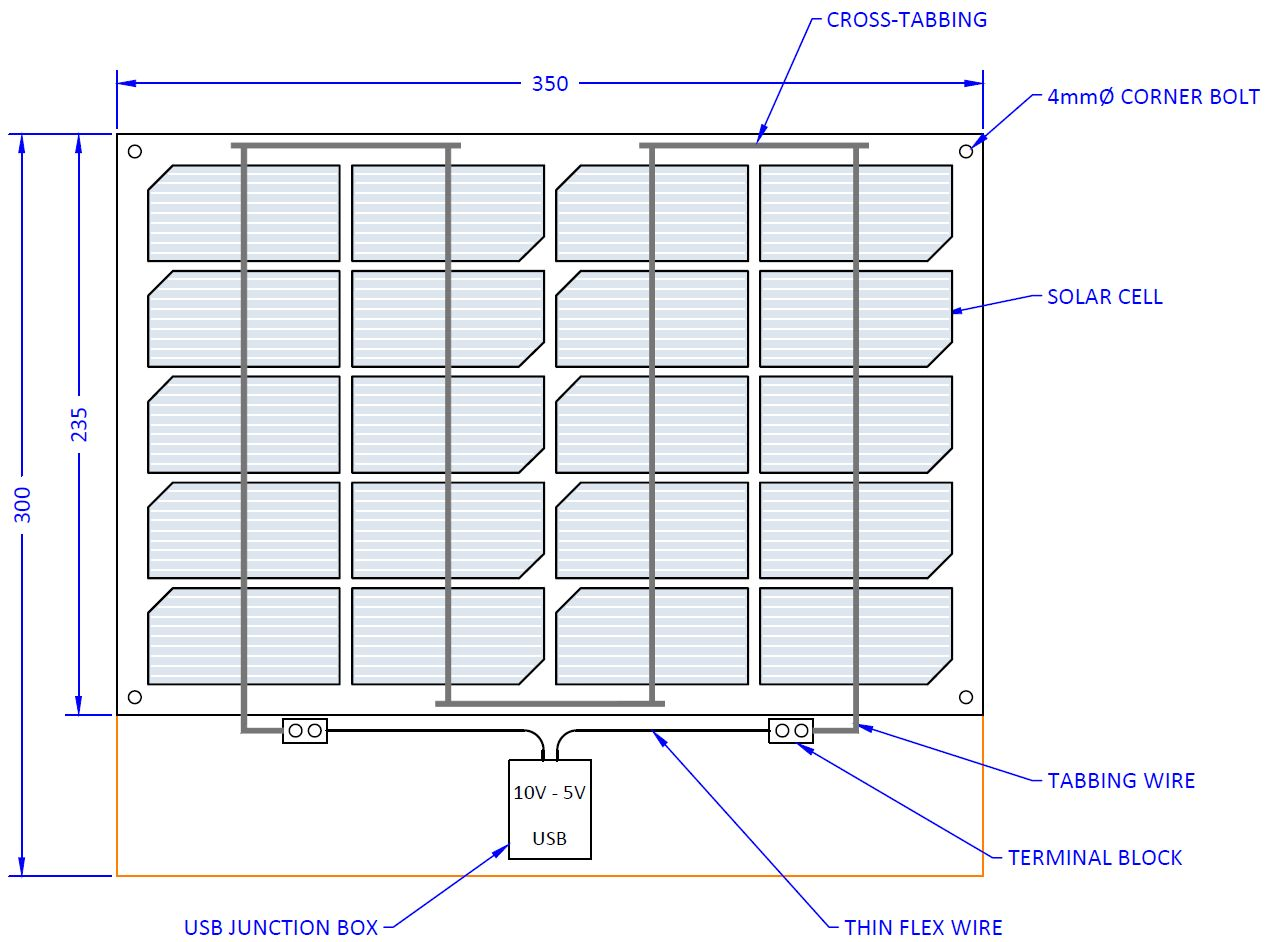
\includegraphics[width=0.8\paperwidth]{Images/image_3_19_(topdown_diagram).png}
    \end{center}

    \begin{center}
      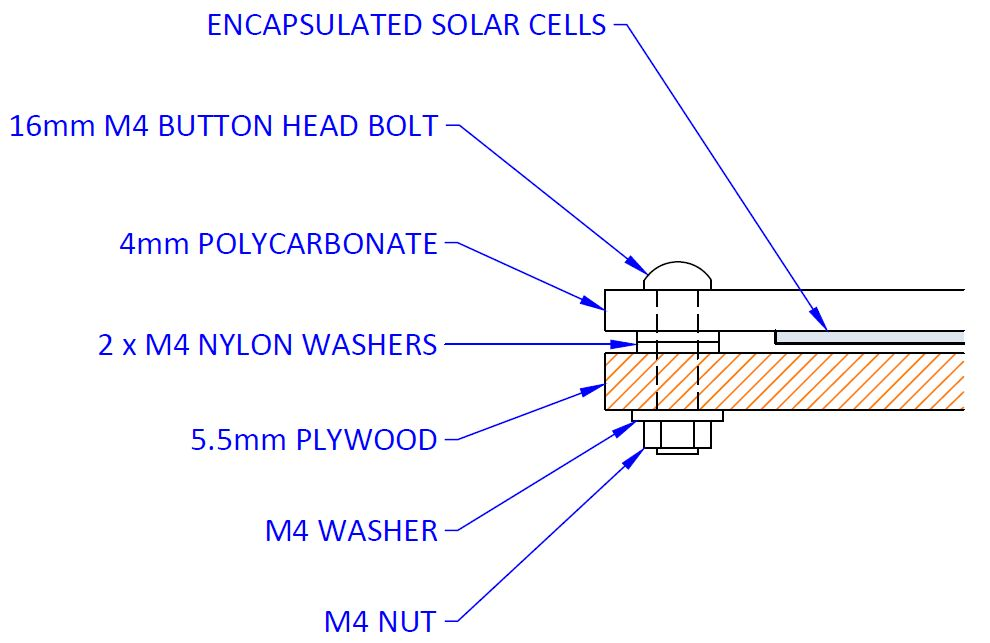
\includegraphics[width=0.4\paperwidth]{Images/image_3_20_(sideview_diagram).png}
    \end{center}
  
  % subsection step_8_attach_usb_dc_dc_voltage_converter (end)

% section building_the_panel (end)

\newpage

\section{Appendix 1: Sourcing materials (and possible alternatives)} % (fold)
\label{sec:appendix_1_sourcing_materials_and_possible_alternatives_}

  \subsection{Solar cells} % (fold)
  \label{sub:solar_cells}

    DEE uses reclaimed 6” square cells that are cut down into regular 1/8th size pieces prior to the workshop. This removes damaged sections of the cells and makes it easier to construct a panel of modest size with a sufficient charging voltage. 

    DEE can supply cells already cut to these sizes on request, but you can cut your own using a rotary tool (Dremel) with a fine diamond-tipped cutting disk. It works best if built into a jig to make a mini-table saw, that allows you to cut stacks of a dozen cells at a time. The cutting process creates a lot of dust, debris and noise, so goggles, ear protectors, and a dust mask are essential. Contact us if you'd like more details on how to do this.

    DEE has 1kW boxes of undamaged 6” x 6” Grade A cells for sale, and can cut them into halves, quarters or eighths as required. Contact us at \href{mailto:info@dee.org.uk}{info@dee.org.uk} with any requests.

    You can also find cells of various sizes and specifications being sold on eBay, which can be useful for smaller projects.
  
  % subsection solar_cells (end)

  \subsection{Polycarbonate} % (fold)
  \label{sub:polycarbonate}

    DEE uses 330mm x 265mm sheets of 4mm thick polycarbonate as the protective front of the solar panel. Polycarbonate is a tough, transparent plastic, that can be made UV resistant, meaning it can be left outside in sunlight for years without degrading. Polycarbonate usually comes in large sheets that will need to be cut to the size you want, but you can order polycarbonate pre-cut to a pre-determined size from a website such as \href{https://www.cutplasticsheeting.co.uk/clear-acrylic-sheeting/clear-polycarbonate-sheet}{https://www.cutplasticsheeting.co.uk/} if needed.

    To cut polycarbonate, it's best to use a table saw, but a powerful jig saw or angle grinder with an appropriate blade or cutting disk will also do the job. As for any type of cutting work, goggles are essential.

    When ordering polycarbonate, ensure that it's UV resistant. Other types of clear plastic such as acrylic or polystyrene are not UV resistant, meaning they will discolour if left in sunlight for too long, so are unsuitable for use in solar panels.

    Glass can be used, but cutting it to the size for this design is difficult, and the EVA doesn't bind as firmly. For alternative designs for larger panels using reclaimed glass windows, see previous versions of DEE workshop guides.
  
  % subsection polycarbonate (end)

  \subsection{EVA} % (fold)
  \label{sub:eva}

    Ethylene Vinyl Acetate (EVA) is used to encapsulate the cells to make them weatherproof and to bind the cells to the polycarbonate sheet and into the neoprene case. It's used for the same purpose in commercially made panels. EVA comes in rolls as a translucent film, but when heated it becomes clear and transparent.

    DEE uses EVA sheets cut from 1m wide rolls, that we can cut to whatever size is needed for our panels.

    It's not the sort of thing that is commonly available to buy, but it is possible to find smaller quantities of solar EVA film on eBay.

    You can also use a specialist two-part epoxy such as Qsil to encapsulate solar cells, but it wouldn't be suitable for this design. For alternative designs for larger panels using Qsil as an encapsulant, see previous versions of DEE workshop guides.
  
  % subsection eva (end)

  \subsection{Tabbing wire} % (fold)
  \label{sub:tabbing_wire}

    Tabbing wire is thin, flat conductive wire that is coated in a layer of solder. 

    DEE has several long reels of 2mm tabbing wire that we use for our workshops, and we can supply it in various lengths.

    Tabbing wire can be ordered on eBay and several other websites in large and small quantities. 
  
  % subsection tabbing_wire (end)

  \subsection{Flux pens} % (fold)
  \label{sub:flux_pens}

    Flux is used to clean the surface of the metallic contacts of solar cells and to help the molten solder flow into the microscopic crevices of the material being soldered onto to create a strong bond.

    DEE uses liquid flux, applied with refillable watercolour brush pens. 

    For small solar panel soldering jobs, you can can also use a disposable flux pen. These are readily available on ebay.

  % subsection flux_pens (end)

  \subsection{DC converters} % (fold)
  \label{sub:dc_converters}

    The DC voltage converter is used to step down the incoming voltage from the solar panel to a stable 5v voltage for a USB output. 

    The DC converters DEE use are enclosed buck converters that are reasonably cheap, efficient, sturdy and waterproof, but there are plenty of other options available that do a similar job. E.g. you could wire in a cigarette lighter socket and use a plug-in USB charger... this would allow you to use the solar panel to supply power to other 12V devices that use a cigarette lighter plug. You could also use an LM7805 voltage regulator, but it would need a decent heat sink to be used with a 12V supply for any length of time.

    These are all readily available from eBay and other online shops. 
  
  % subsection dc_converters (end)

  \subsection{USB Battery packs} % (fold)
  \label{sub:usb_battery_packs}

    DEE recommends using a USB power bank with a solar charger to make best use of it. Having a power bank battery gives you the option to store energy that you can use to recharge your devices at night, instead of only using the solar power to charge devices directly when the sun is out.

    One of the other workshops run by DEE shows how to make a USB power bank using lithium cells recovered from old laptop batteries. See \href{https://www.demandenergyequality.org/our-workshops}{our workshops} page for details.

    In good direct sunlight, a 12W solar charger should be able to charge up a mobile phone or a 2000mAh battery pack in 2 hours. Bigger USB battery packs are available if you are looking for more storage.

  % subsection usb_battery_packs (end)

% section appendix_1_sourcing_materials_and_possible_alternatives_ (end)

\end{document}